 \documentclass[ngerman]{scrartcl} %lädt die Dokumentklasse
                                %Artikel von Koma-Skript, als Option
                                %übergebe ich, dass ich die Trennung
                                %nach neuer deutscher Rechtschreibung
                                %wünsche
\usepackage[utf8]{inputenc}
 \usepackage[ngerman]{babel}
\usepackage{color}
\usepackage[T1]{fontenc}
\usepackage[pdfborder={0 0 0}]{hyperref}
\usepackage[a4paper,lmargin={4cm},rmargin={2cm},
tmargin={2.5cm},bmargin = {2.5cm}]{geometry}
\usepackage{amssymb}
\usepackage{graphicx}
\usepackage{amsthm}
\usepackage{graphicx}
\usepackage{url} 

\begin{document}
\tableofcontents
\newpage
 
\section{Einleitung}        
\label{sec:Einleitung-1}   

In den letzten Jahren konnten aufgrund technologischer Entwicklungen immer mehr Geräte entwickelt werden, die in den verschiedensten Bereichen des täglichen Lebens eingesetzt werden. Diese Entwicklungen betreffen dabei meist die Leistungsfähigkeit, Konnektivität oder Größe der Geräte, sodass sie in immer mehr und unterschiedlicheren Bereichen eingesetzt werden können. Ein Begriff der in den letzten Jahren für dieses Phänomen immer häufiger genutzt wurde, ist das ``\ac{IoT}'' zu deutsch ``Das Internet der Dinge''. Mit dem \ac{IoT} wird beschrieben, dass immer mehr Geräte mit dem Internet verbunden sind und Daten austauschen. Im Rahmen dieser Entwicklung sind verschiedenste Nutzungsszenarien umgesetzt worden, die das tägliche Leben erleichtern oder automatisieren sollen. Diese Studienarbeit wird sich im folgenden mit einem speziellen Szenario befassen, welches unter anderem durch den Onlinehändler Amazon umgesetzt wurde.

Das Szenario umfasst sogenannte ``Amazon Dash Buttons''. Diese Buttons sind kleine Geräte, welche an unterschiedlichen Stellen in der Wohnung des Kundens angebracht werden können und über einen Druckknopf verfügen. Nach einer Konfiguration durch den Benutzer kann mithilfe eines Drucks auf den Sensor ein zuvor ausgewähltes Produkt bestellt werden. Ein Beispiel wäre das nachbestellen von Waschpulver. So könnte der Button an der Waschmaschine befestigt sein und bei einem geringen Vorrat an Waschpulver wird der Button betätigt und das ausgewählte Waschpulver innerhalb der nächsten Tage geliefert. So entfällt für den Nutzer der händische Bestellvorgang, da dieser automatisch durch den Button und Amazon durchgeführt wird. Dieses Beispiel lässt sich natürlich auf verschiedene andere Möglichkeiten übertragen, so könnten auch Dinge, wie Kaffee, Zahnpasta, Tierfutter, Getränke oder ähnliches nachbestellt werden. Dem Nutzer wird eine Vereinfachung des Kaufprozesses versprochen und der Händler bindet den Kunden stärker an sich, da der Button direkt bei Amazon bestellt. 
Die Studienarbeit setzt sich zum Ziel eine Untersuchung des Amazonproduktes durchzuführen und die Machbarkeit und Umsetzung einer offeneren Lösung zu prüfen. 

    

\newpage

\section{Überblick der vorgestellten Lösung}
\label{sec:Überblick der vorgestellten Lösung-1}
Die vorgestellte Lösung soll auf freie Technologien zurückgreifen und somit für den Nutzer nachvollziehbar sein. Das erklärte Ziel ist es, über Buttons einen Einkaufszettel zusammenzustellen, der dem Nutzer dann zur Verfügung gestellt wird. Dazu wird mit sogenannten Mikrocontrollern und Einplatinencomputern die benötigte Infrastruktur realisiert und aufgebaut. Damit die Daten nicht außerhalb der Kontrolle des Nutzers liegen, wird ein zentraler Server im Netzwerk benötigt. Dieser zentrale Server empfängt zudem die entsprechenden Signale der Clients, die in diesem Falle die Buttons sind. 

\newpage

\section{Theorie}        
\label{sec:Theorie-1}  

\subsection{UDP}
\label{sec:UDP-1}

\ac{UDP} steht für ``User-Datagram-Protocol'' und ist ein verbindungsloses Transportprotokoll. Im \ac{OSI}-7-Schichten Modell arbeitet es auf der Transportebene und ist für die Zustellung von Netzwerkpaketen von einem Sender zu einem Empfänger zuständig. Im Vergleich zum Transportprotokoll \ac{TCP}, welches verbindungsorientiert arbeitet, ist es wesentlich einfacher zu verarbeiten, da beispielsweise der Header bei den einzelnen Datenpaketen wesentlich kleiner ist. Allgemein ist es sehr minimal gehalten und dadurch sehr einfach zu implementieren und für sehr einfache Anwendungszwecke geeignet. Allerdings ist auch zu erwähnen, dass es keine Empfangsbestätigung gibt und die Daten nach dem Absenden nicht weiter kontrolliert werden. Somit können die Daten auch im Netzwerk verloren gehen und es wird nicht bemerkt. \\
Der einfache Header des \ac{UDP} Protokolls besteht nur aus vier Attributen. Diese jeweils 16 Bit großen Felder enthalten den Quellport, den Zielport, die Checksumme zur Überprüfung des Inhalts und die Länge des gesamten Pakets. Insgesamt ist der Header somit 8 Byte groß. (vgl. \cite{ElektronikKompendium.}\cite{.}\cite{.23.02.2016})
 

\subsection{TCP}
\label{sec:TCP-1}

\ac{TCP} ist ein verbindungsorientiertes Protokoll, dass im \ac{OSI}-7-Schichten Modell auf der vierten Ebene (Transport) einzuordnen ist. Im sogenannten \ac{TCP}/\ac{IP} Protokollstapel ist es in der dritten von vier Schichten zu finden. Bei einer Übertragung von Daten über \ac{TCP} übergibt die genutzte Anwendung den Datenstrom an das Protokoll und empfängt ihn auch wieder von dort. Für die Übertragung ist dementsprechend \ac{TCP} zuständig. 
Die Hauptaufgaben des Protokolls sind daher die Aufteilung und die Zusammensetzung der Daten von entsprechend vielen Paketen (Segmentierung), das Management der Verbindung und ein entsprechendes Fehlerhandling, welches das korrekte Empfangen von Paketen überwacht. Das Fehlerhandling nutzt eine positive Bestätigung aller Pakete. Dies bedeutet, dass nur nicht vorhandene Pakete erneut angefragt werden, ansonsten davon ausgegangen wird, dass die Daten beim Empfänger angekommen sind. Diese Technologie sorgt dafür, dass die Daten auf jeden Fall ankommen, sofern die Verbindung nicht gestört wird (vgl. \cite{.c}\cite{.22.11.2016}).

Der Header eines \ac{TCP} Pakets besteht aus 20 Bytes, jedoch kann dieser auch noch erweitert werden, sodass noch einige zusätzliche Bytes in den Header geschrieben werden. Zu den zwingend notwendigen Daten gehört unter anderem der Port auf dem das Paket empfangen wird und der Port über den das Paket gesendet wird. Zudem wird die Nummer im aktuellen Paketstrom benötigt. Zudem wird eine Prüfsumme und Quittierungsnummer mitgegeben, welche zur Kontrolle und Bestätigung genutzt werden (vgl \cite{.c}).


\subsection{Webserver: Nginx}
\label{sec:Webserver: Nginx-1} 
 
\subsection{Arduino}
\label{sec:Arduino-1} 

\subsection{WLAN-Chipsatz}
\label{sec:WLAN-CHipsatz-1} 

\subsection{Frontendtechnologien}
\label{sec:Frontendtechnologien-1}
 
\subsection{REST}        
\label{sec:REST-1}  

\cite{Tilkov.2015}
  
\newpage
 
\section{Auswahl der Hardware}        
\label{sec:Auswahl der Hardware-1}  

In den folgenden Kapiteln wird die ausgewählte Hardware des Projektes vorgestellt. Dabei wird zuerst auf die technischen Merkmale eingegangen und dann auf den genauen Verwendungszweck im Projekt. 

\subsection{Raspberry PI}        
\label{sec:Raspberry PI-1} 


\subsubsection{Vorstellung des Raspberry PI}        
\label{sec:Vorstellung des Raspberry PI-1} 

Das Raspberry PI ist ein Einplatinencomputer, den es in verschiedenen Ausführungen gibt. Je nach Ausführung variieren die Ausstattungsmerkmale. Zu den Grundsätzlichen Ausstattungsmerkmalen gehören eine CPU, unterschiedlich viel RAM und eine iGPU Einheit. Er wurde von der Raspberry PI Foundation entwickelt und hatte das ursprüngliche Ziel einen günstigen Computer für den Schulunterricht bereitzustellen. Daher ist es auch möglich eine vollständige Linux Distribution als Betriebssystem zu nutzen und es wurde sogar eine speziell angepasste Distribution veröffentlicht, die Raspbian bezeichnet wird. 
Aufgrund der verschiedenen Möglichkeiten wird er aber mittlerweile auch in vielen anderen Anwendungsgebieten genutzt. Insbesondere die neueren Modelle, die mit mehreren USB Ports, \ac{GPIO} Pins, einem Ethernet Port und weiteren Anschlüssen ausgestattet sind, werden auch in verschiedensten Projekten privater Personen genutzt. Ein weiteres Merkmal ist die Größe des Raspberry PI's, die mit maximal 93mmx63.5mmx20mm sehr klein ausfällt. Zusätzlich gibt es diverses, bereits für den Raspberry PI ausgelegtes, Zubehör, welches weitere Erweiterungsmöglichkeiten bietet. So gibt es Kameras, Gehäuse, kleine Displays und WLAN Sticks, die den Funktionsumfang erweitern. So wurden bereits diverse Projekte vorgestellt, die zeigen, dass die Einsatzmöglichkeiten des Raspberry Pis wesentlich größer sind. (vgl. \cite{.28.12.2016} \cite{.28.01.2017})
\\
\begin{figure}[!htb]
	\centering
	\includegraphics[scale=0.5]{Raspberry-Pi-2-web.png}
	\caption[RaspberryPi Modell 2 B]{RaspberryPi Modell 2 B+,\\ Quelle: https://www.raspberrypi.org/wp-content/uploads/2016/02/Raspberry-Pi-2-web.jpg}
\end{figure}


\subsubsection{Verwendung im Projekt}        
\label{sec:Verwendung des Raspberry PI-1} 
Der Raspberry PI wird für das Projekt genutzt, um einen zentralen Server bereitzustellen. Aufgrund der technischen Merkmale kann zeitgleich ein Webserver und ein Datenbankserver betrieben werden. Zudem kann über die USB Anschlüsse ein WLAN Stick angeschlossen werden, sodass die Buttons über das WLAN Netzwerk des Raspberry PIs zum zentralen Server kommunizieren können. Dazu muss mithilfe eines Skriptes der WLAN Stick von einem Empfänger zu einem Sender bzw. Access Point umfunktioniert werden. Um die dann eingehenden Nachrichten der Buttons empfangen zu können, muss zudem noch ein entsprechendes Skript im Hintergrund laufen, dass die Daten empfängt. Aufgrund von mehreren parallel laufenden Prozessen (Webserver, Datenbankserver, WLAN Skript und Skripte zum Empfangen der Daten) wird einiges an Rechenleistung benötigt, die der Raspberry Pi allerdings aufbringen kann. 

Der Webserver auf dem Raspberry Pi wird dabei sowohl für das Frontend als auch für das Backend benötigt werden. Das Frontend soll dem Nutzer die Möglichkeit geben, die Liste von Waren zu verwalten und die Buttons zu konfigurieren bzw. Hilfestellung zur Einrichtung zu geben. Das Backend des Servers wird unter anderem aus einer \ac{REST} \ac{API} bestehen, die sowohl die Anfragen des Webservers verarbeitet als auch die Anfragen an die Datenbank im allgemeinen. 
Der Datenbankserver im Hintergrund wird die benötigte Datenbank entsprechend verwalten. 

\subsection{``Pretzelboard''}        
\label{sec:''Pretzelboard''-1} 

\subsubsection{Vorstellung des ``Pretzelboard''}        
\label{sec:Vorstellung des ``Pretzelboard''} 
Das ``Pretzelboard'' ist ein sogenanntes Elektronikmodul, dass unter verschiedenen Namen bekannt ist. Neben ``Pretzelboard'' ist der Name ``NanoESP-Board'' ebenfalls bekannt. Die Besonderheit des Boards ist ein bereits angeschlossenes WLAN Modul, welches sowohl als Sender als auch Empfänger arbeiten kann. Da es zudem den gleichen Mikrocontroller wie das bekanntere Mikrocontrollerboard ``Arduino Uno'' nutzt, kann die Entwicklungsumgebung von Arduino zur Entwicklung von Software genutzt werden. 
Der Vorteil der bereits erfolgten Kombination und Verdrahtung von WLAN Modul und Mikrocontroller liegt darin, dass der Nutzer dies nicht mehr machen muss und somit wesentlich weniger Kenntnisse vorausgesetzt werden müssen. (vgl. \cite{.b}\cite{.kafka}\cite{FranzisVerlagGmbH.27.11.2015})


\subsubsection{Verwendung im Projekt}        
\label{sec:Verwendung des ``Pretzelboard''} 
Das ``Pretzelboard'' wird im Projekt als Button genutzt. Sowohl die kleine Größe als auch die bereits vorhandene WLAN Funktionalität sorgen dafür, dass sich das Board dafür besonders gut eignet. Aufgrund der Tatsache, dass es sich bezüglich der Programmierung nicht von einem Arduino Board unterscheidet, besteht die Möglichkeit, dass auf das Wissen und den Support einer bereits größeren Community zurückgegriffen werden kann. 
Da sich das Board zudem auf ein Elektroniksteckboard setzen lassen kann, ist auch die Verbindung mit einem Button und Statusleuchten möglich. Nach der erfolgreichen Montage kann dann das entsprechende Programm aufgespielt werden und bei vorhandener Stromversorgung kann die entsprechende Nachricht über das WLAN Netzwerk an den Empfänger gesendet werden. Das Pretzelboard kommuniziert diese Nachricht mithilfe des zuvor bereits erwähnten Protokolls \nameref{sec:UDP-1}.

\begin{figure}[!htb]
	\centering
	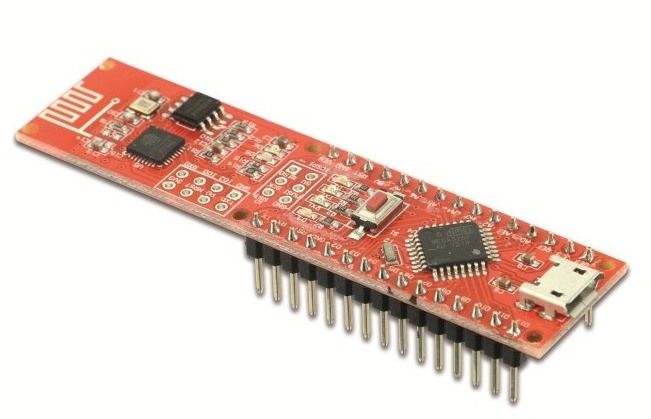
\includegraphics[scale=0.4]{pretzel.jpg}
	\caption[``Pretzelboard'']{``Pretzelboard'',\\ Quelle: http://cdn.pollin.de/article/xtrabig/X880281.2.JPG}
\end{figure}

\newpage


\section{Umsetzung des Projektes}        
\label{sec:Umsetzung des Projektes-1}  

\subsection{Architektur und Zusammenspiel der Komponenten}        
\label{sec:Architektur und Zusammenspiel der Komponenten-1} 

Einbindung von \nameref{sec:Auswahl der Hardware-1}

\subsection{Einrichtung der Hardware}  
\label{sec:Einrichtung der Hardware-1} 

\subsubsection{Einrichtung des Raspberrys}  
\label{sec:Einrichtung des Raspberrys-1}

\paragraph{Einrichtung des WLAN Access Points}  
\label{sec:Einrichtung des WLAN Access Points-1} 

\paragraph{Einrichtung des UDP Empfängers}  
\label{sec:Einrichtung des UDP Empfängers-1} 

\subsubsection{Einrichtung des ``Pretzelboards''}  
\label{sec:Einrichtung des ``Pretzelboards''-1}

\subsection{Entwicklung der Webanwendung}  
\label{sec:Entwicklung der Webanwendung-1} 

\subsubsection{Aufbau und Entwicklung der REST API}  
\label{sec:Aufbau und Entwicklung der REST API-1}

\subsubsection{Aufbau und Entwicklung des Frontends}  
\label{sec:Aufbau und Entwicklung des Frontends-1}

\subsection{Entwicklung und Einrichtung der Datenbank}  
\label{sec:Entwicklung und Einrichtung der Datenbank-1} 

\newpage

\section{Ergebnis des Projektes}        
\label{sec:Ergebnis des Projektes-1}  

\newpage

\section{Fazit und Ausblick}        
\label{sec:Fazit und Ausblick-1}  

\newpage


\addcontentsline{toc}{section}{Literaturverzeichnis}
\bibliographystyle{unsrt}  
\bibliography{Literatur}

\newpage

\addcontentsline{toc}{section}{Abbildungsverzeichnis}

\listoffigures

\end{document}